\PassOptionsToPackage{unicode=true}{hyperref} % options for packages loaded elsewhere
\PassOptionsToPackage{hyphens}{url}
%
\documentclass[]{article}
\usepackage{lmodern}
\usepackage{threeparttable}
\usepackage{geometry}
\usepackage{amssymb,amsmath}
\usepackage{ifxetex,ifluatex}
\usepackage{fixltx2e} % provides \textsubscript
\usepackage{hyperref}
\usepackage{graphicx,grffile}
\usepackage{tabularx}
\usepackage{longtable}
\usepackage{paralist}

\usepackage{lscape}
\usepackage{booktabs, multirow} % for borders and merged ranges
\usepackage{soul}% for underlines
\usepackage[table]{xcolor} % for cell colors
\usepackage{changepage,threeparttable} % for wide tables
\usepackage{cite}

\ifnum 0\ifxetex 1\fi\ifluatex 1\fi=0 % if pdftex
\usepackage[T1]{fontenc}
\usepackage[utf8]{inputenc}
\usepackage{textcomp} % provides euro and other symbols
\else % if luatex or xelatex
\usepackage{unicode-math}
\defaultfontfeatures{Ligatures=TeX,Scale=MatchLowercase}
\fi

% use upquote if available, for straight quotes in verbatim environments
\IfFileExists{upquote.sty}{\usepackage{upquote}}{}
% use microtype if available
\IfFileExists{microtype.sty}{%
	
	\usepackage[]{microtype}
	\UseMicrotypeSet[protrusion]{basicmath} % disable protrusion for tt fonts
}{}

\IfFileExists{parskip.sty}{%
	\usepackage{parskip}
}{% else
	\setlength{\parindent}{0pt}
	\setlength{\parskip}{6pt plus 2pt minus 1pt}
}

\hypersetup{
	pdfborder={0 0 0},
	breaklinks=true}
\urlstyle{same}  % don't use monospace font for urls
\setlength{\emergencystretch}{3em}  % prevent overfull lines
\providecommand{\tightlist}{%
	\setlength{\itemsep}{0pt}\setlength{\parskip}{0pt}}
\setcounter{secnumdepth}{0}
% Redefines (sub)paragraphs to behave more like sections
\ifx\paragraph\undefined\else
\let\oldparagraph\paragraph
\renewcommand{\paragraph}[1]{\oldparagraph{#1}\mbox{}}
\fi
\ifx\subparagraph\undefined\else
\let\oldsubparagraph\subparagraph
\renewcommand{\subparagraph}[1]{\oldsubparagraph{#1}\mbox{}}
\fi

\renewcommand{\baselinestretch}{1.75}

\renewcommand{\arraystretch}{5}


\newgeometry{vmargin={15mm}, hmargin={30mm,30mm}}   % set the margins 


% set default figure placement to htbp
\makeatletter
\def\fps@figure{htbp}
\makeatother


\newcommand{\pplfont}[1]{{\textbf{\fontfamily{ppl}\selectfont #1}}}

\newcommand{\lmttfont}[1]{{\fontfamily{lmtt}\selectfont #1}}


\begin{document}

\section*{Radiomics}\label{radiomics}

\subsection*{Introduction}\label{introduction}

As explained previously, there are globally two ways for establishing a
diagnosis of diseases such as liver cancers: the biopsy, or the
diagnostic imaging.

The biopsy, as detailed earlier, suffers from a lot of drawbacks. It
remains an invasive procedure, with a high cost in terms of resources,
and does not consider the tumor heterogeneity.

The diagnostic imaging on the other hand, is not invasive, provides
information about the tumor shape, the growth over the time, and is less
prone to bias due to tissue heterogeneity.

The recent improvements in the medical imaging field allow acquisition
of data being more and more relevant, thus enabling a better estimation
of the phenotypical characteristics of the patients.

In the case of brain imaging, the augmentation of contrast, on MR
images, thanks to the injection of contrast agents such as
gadolinium-based agents (method mentioned before) is an important
technique for the evaluation of brain and liver tumors \cite{Drevelegas2011,Zhou2014,Thian2013}. This tool allows a delineation of large tumors and an
early detection of small metastatic lesions. The different MRI sequences
(e.g. the T1 weighted sequences) also allow an internal separation of
the tissue within the same tumor (active vs necrotic part of the tumor)
\cite{Drevelegas2011}.

Support brought by the innovations in the medical imaging field have
been demonstrated on other organs such as the liver \cite{Davnall2012}, the breast \cite{Koolen2012} or the colon
\cite{Sahani2014} with a consequent benefit in terms of
diagnosis.

However, even though the advancements in the medical imaging fields
allowed those performances, the interpretation of the medical images
remains subjective and not quantitative. In order to correctly provide a
diagnosis that will not depend on the observer, one can extract and use
the characteristics previously difficult, even impossible to distinguish
with the naked eye.

Introduced in the 80s, \emph{CAD} (Computer Assisted Diagnosis) tools
were the first to implement this method, to establish a link between the
imaging features and the biological characteristics of the patients
\cite{Doi2007}.

In order to go along with those new systems, standard were introduced
such as the one created by the \emph{WHO} or the \emph{RECIST}
\cite{Jaffe2006}, were the objective was to assess the
evolution of the disease following the progression of the tumor size,
but here again, those criteria suffer from a too high dependence with
the observers.

The term \emph{radiomics} was introduced in the early 2010s, allowing
the computation of more features than the traditional \emph{CADs} (more
than a thousand vs only a dozen previously) and bringing a more complete
diagnosis, since \emph{CADs} were often limited to distinguish benign vs
malignant lesions \cite{Afshar2018}.

This new technique allows some breakthroughs in various applications
such as the cancer diagnosis, the detection of the tumors (with the
identification of malignant lesions), their classification, the
estimation of the patient survival, the prediction of the aggressivity
of the tumors, their recurrence, or the advancement of the disease.

In the clinical practice, this new method also allows an improvement in
the way biopsies are performed, with the identification of the areas
where the extraction should be performed \cite{Gillies2016}
or even by prediction when a biopsy is helpful or not \cite{Liu2016}.

Compared to above-mentioned criteria based on a naked-eye examination,
we are now able to rely on a computer to analyse the gray-levels at a
finer scale. Therefore, 2 approaches exist, the \emph{HCR} (Hand-Crafted
Radiomics) based on mathematical engineered features, relying on the
textural and intensity based properties of the volume of interest, and
the \emph{DLR} (Deep-Learning radiomics), where the retained features
will directly be computed from the input data without any prior
knowledge.

\subsection{Handcrafted Radiomics }\label{handcrafted-radiomics}

In this section we will describe the \emph{HCR} pipeline, by first
exposing the different steps of the classical workflow, before analysing
the different studies that used \emph{HCR} on patients suffering from
\emph{HCCs}. We will conclude with the different improvements that
should be brought to enhance the power of radiomics.

A conventional radiomics workflow (based on \emph{HCR} features) starts
with the acquisition and the reconstruction of medical images, followed
by the segmentation of those images, which is a critical step since
\emph{HCR} features are extracted from the segmented sections, and many
tissues do not have distinct boundaries \cite{Gillies2016}. Once the different areas segmented, the features are
extracted and quantified, and a statistical analysis is performed to
select only the most relevant one. The final step consists in building a
model that will use the selected features to perform the wanted task,
which is often either the tumor characterization or its prognosis. The
pipeline is illustrated in the figure below \ref{Scrivener2016_Fig1}.


\begin{figure}[th!]
\centering
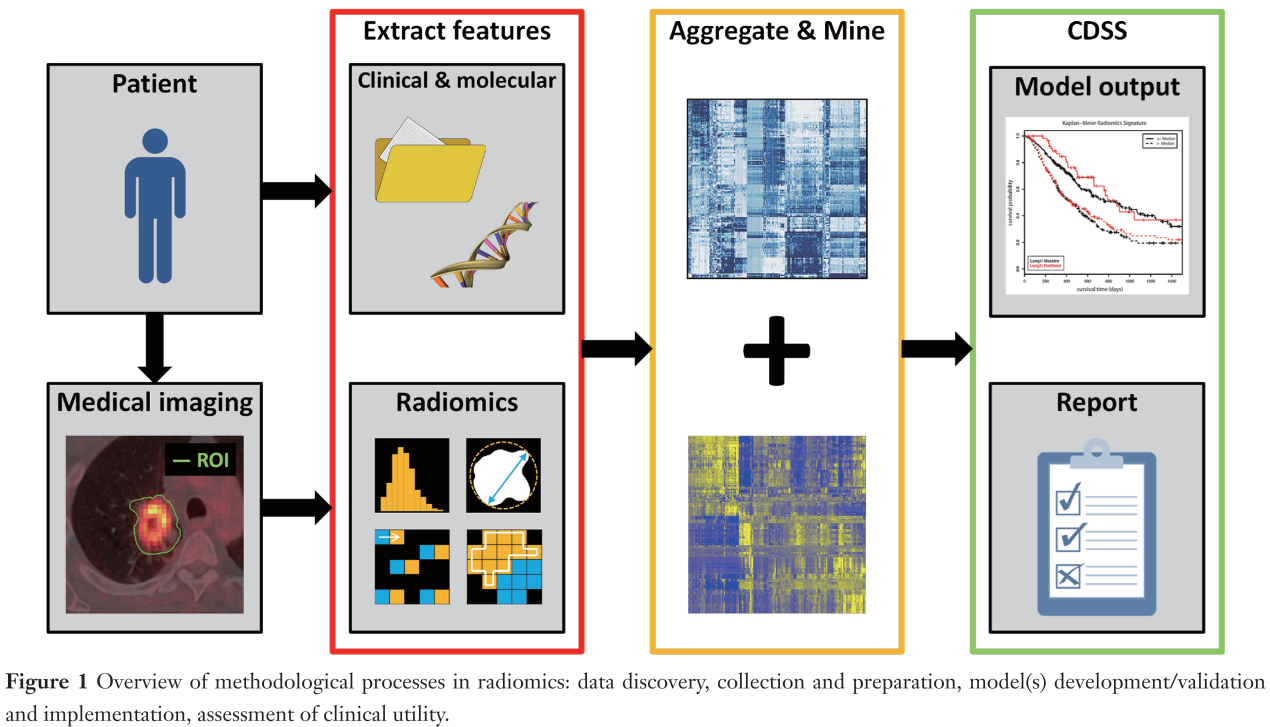
\includegraphics[width=0.7\linewidth]{images/image4}
\caption{Radiomics classical workflow as depicted by ©Scrivener et al. \cite{Scrivener2016}}
\label{Scrivener2016_Fig1}
\end{figure}


We will now describe those different steps, before analyzing recent
state-of-the-art \emph{HCR} studies, before establishing a list of
measures needed to be taken in order to improve the quality and the
reproducibility of future radiomics works.

\subsubsection*{HCR workflow}\label{hcr-workflow}

As explained previously, ultrasonography (US) is the recommended
modality as primary imaging test for surveillance. If the surveillance
is positive, CT or MR examinations are performed for the diagnosis and
the staging of the disease. For the reasons exposed previously, namely
the availability, and its robustness when compared to MRI, we will focus
on \emph{HCR} studies based on CT imaging data.

Without entering into the details of how a CT scan works, we can assume
that performances of the CT imaging depend mainly on some settings such
as the slice thickness, the capability for projecting the density
variations into image intensities and the reconstruction algorithm which
aims at converting tomographic measurements into cross-sectional images.

It has been demonstrated that radiomics features can differ between
different scanners with the same settings \cite{Berenguer2018}. It is also common to differentiate CT images into two
categories, the screening where low dose images are used and the
diagnosis with higher quality of contrast obtained with higher doses \cite{Thawani2018}. Worth mentioning that the
majority of the studies that are being investigated belong to the second
category.\\
Images are typically combined with other clinical sources when computing
the radiomics features. Among them, gene expressions, clinical data such
as the age, the gender or the past medical history, blood biomarkers or
other prognostic markers such as the tumor size, the stage or the
recurrence are the main non-imaging sources of data that are used in the
radiomics workflow. However, they can be difficult to acquire, normalize
and integrate in a radiomics pipeline, therefore, features are most
commonly extracted from images only.

\paragraph{Segmentation}\label{segmentation}

Historically, the segmentation was performed manually, hence, sensitive
to the inter-observer variability, as depicted below {[}\textbf{ref
Echegaray et al. 2015, ref Bakr et al. 2017}{]}.

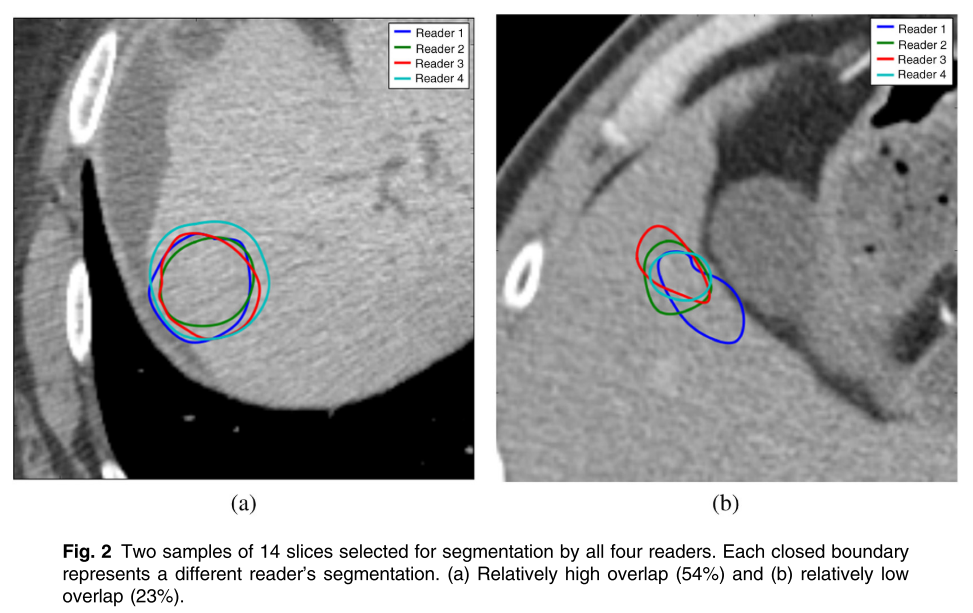
\includegraphics[width=4.92776in,height=3.10385in]{./images/image11.png}

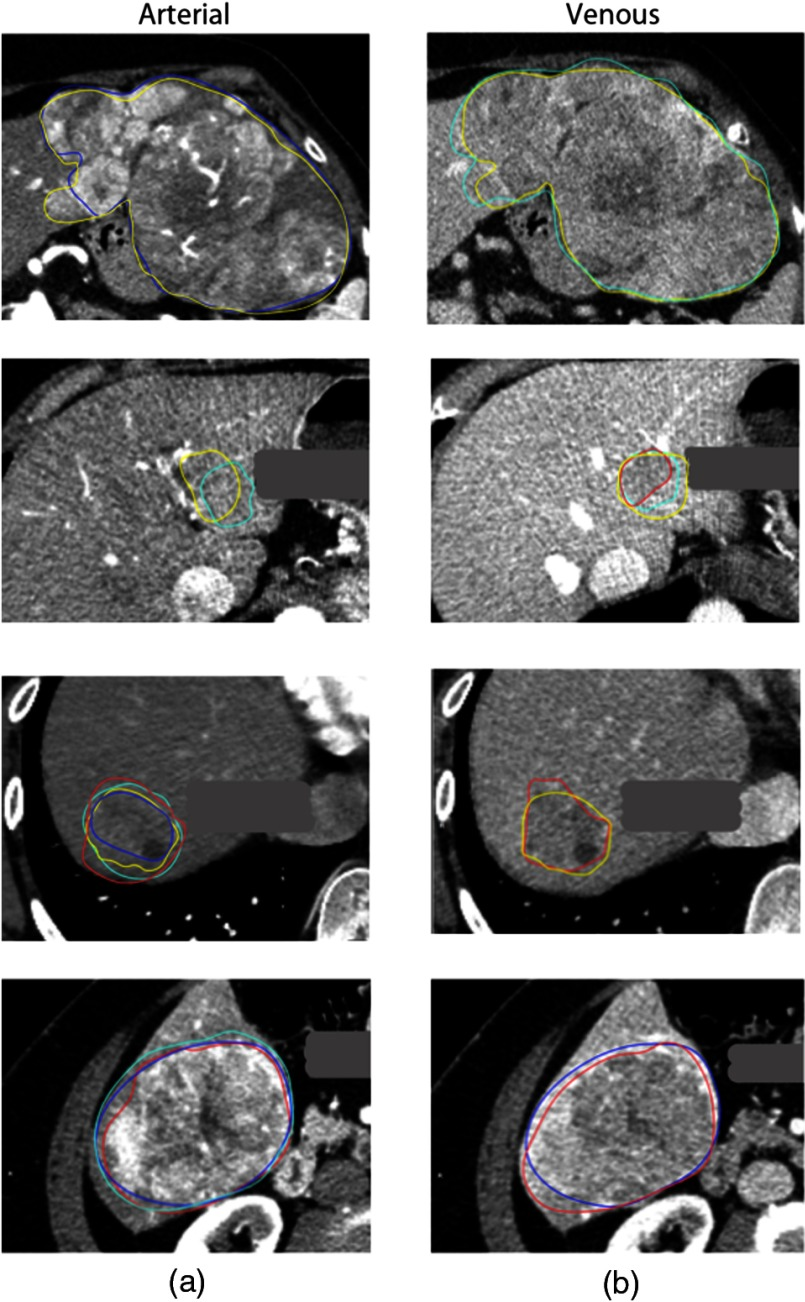
\includegraphics[width=4.22775in,height=6.83726in]{./images/image14.png}

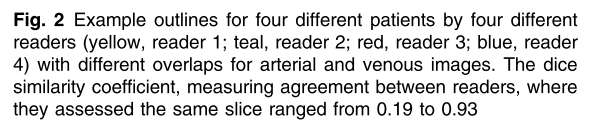
\includegraphics[width=4.26141in,height=0.87100in]{./images/image9.png}

To reduce this bias, semi-automatic segmentation techniques were
developed. Those based on the intensity of the pixels suffer from the
fact that the intensity of the pixels, in the case of abdominal organs,
is often close from one organ to another. On the other hand, models
based on statistical models often require the computation of an energy
function, that can involve a large number of parameters, thus being
difficult to compute and optimize.\\
(More details concerning the liver semantic segmentation techniques can
be found in the appropriate section {[}\textbf{see Sem. Seg.
chapter}{]}).\\
Once the volume of interest delineated, different features can be
extracted. On one hand, features can be chosen a priori for their
capacity to translate the physiological behavior expected by the
experts. For example, studies performed on the lungs showed a
correlation between the textural homogeneity and the survival of the
patients {[}\textbf{ref 17, 18 of HT report}{]}, or the grade
{[}\textbf{ref 19}{]}. This knowledge can also be used in the case of
brain tumors to assess the response to a treatment, by observing for
example the vascular or cellular density {[}\textbf{ref 20, 7 HT
report}{]}. However, a prior knowledge is not always for the wanted
task, therefore, the alternative is to extract a huge quantity of
features and to determine the most relevant one by using for example
some machine learning algorithms.

\paragraph{Features}\label{features}

Features can be regrouped into different categories depending on their
statistical order (first, second or higher order). For the features
belonging to the first statistical order, the volume of interest is
transformed into an histogram, and different values are computed such as
the uniformity or the entropy. Even though those features are often
sensitive to the acquisition settings such as the slice thickness or
even the way the histogram is computed, they permitted the prediction of
the malignancy of breast lesions {[}\textbf{ref 21 of HT report}{]}.\\
Shape features are often extracted directly from the VOI in order to
analyze its geometrical properties (such as the overall volume occupied
by the tumor, its sphericity, its roughness or its fractal dimension).
Those features also permitted the prediction of the response to
treatment in previous studies {[}\textbf{ref 22 of HT report}{]}.

Second order statistical features are meant to extract the textural
properties of the volume, by considering the neighboring relationship
between pixels. This will play an important role especially for the
characterization of the heterogeneity of the tissues. This relation is
captured by several descriptive matrices (\emph{GLCM}, \emph{GLRLM},
\ldots{}) {[}\textbf{ref 21 of HT report}{]}.\\
Finally, higher order features allow the extraction of imaging features
in various frequency domains (the Wavelet features are the most commonly
used higher order features {[}\textbf{ref 22 of HT report}{]}).

\paragraph{Features Selection}\label{features-selection}

As listed here, a large quantity of features can be extracted and they
tend sometimes to be highly correlated, which in some cases can cause
overfitting during the creation of a predictive model. A diminution
phase of the number of features is often required, either in a
supervised manner (features are selected for their discriminant power in
regards with the wanted task) or in non-supervised manner (the main
objective is to suppress the redundant features without considering the
different labels) {[}\textbf{ref 21 HT report}{]}.

Among the supervised methods, one can distinguish the univariate ones,
where the features are tested one by one depending on their contribution
to the wanted task (Wilcoxon or Fisher test), from the multivariate
where the features are regrouped into subsets before being tested
against the output class.

Unsupervised methods (such as the \emph{PCA}: principal component
analysis) are less prone to overfitting since they do not consider the
label of the data, but their main goal is to reduce the dimensionality
of the features space.

Once the number of features is reduced, the next step is to construct a
predictive model, by using either clustering methods (patients are
regrouped based on a metric depending on the retained features) or
classification ones (where models such as \emph{RF}: random forests or
\emph{SVM}: support vector machines are trained from the selected
features in order to predict the wanted clinical criteria). Concerning
the prediction of the survival, it is common to implement slightly
different models such as the \emph{Kaplan-Meier} or the \emph{Cox
Proportional Hazard} {[}\textbf{ref 23 HT report}{]}.

In the radiomics studies, one of the main goals is the stability of the
features against the pre-treatment steps described above. In order to
reach this objective, it is possible for the patients to undergo the
medical imaging examinations several times (\emph{test-retest}), and the
segmentations can be performed by several experts or even by the same
expert several times {[}\textbf{ref 24 HT report}{]}.

In summary, when dealing with classical radiomics pipelines, reaching
the best results will often depend on the best combinations between the
extraction of the features, the technique used to reduce the number of
features and the method implemented to create the model.

Every modification on the cited steps can have a huge impact on the
predictable performances of the created model.

In the next section, we will analyze the different \emph{HCR} studies
performed on patients suffering from \emph{HCC} and who underwent CT
examination. We will first describe the different choices made in each
step of the classical pipeline, before presenting ways to improve the
quality of future \emph{HCR} work.

\subsubsection{HCR applied to the liver}\label{hcr-applied-to-the-liver}

In order to analyze the different methods implemented in the \emph{HCR}
field, 15 studies performed on patients suffering from HCC and who
underwent CT scan examination were reviewed. Initially, 23 primary liver
cancer-related studies have been scanned in our review {[}\textbf{ref
TAIGA}{]}, we then selected the 15 HCC-related ones.

We will first describe the different targets of the studies and the
details of the cohorts through the number of patients and the clinical
criteria that preceded their selection.

We will then compare the different imaging acquisition protocols, and
the way the regions/volumes of interest are delineated. Finally, we will
analyze the different features that appeared to be relevant in the
studies, before proposing some tracks to improve the reproducibility and
the performances of future radiomics work.

Details concerning the experimental settings of the studies, the
endpoints and the different endpoints can be found in the following
table
(\href{https://docs.google.com/spreadsheets/u/0/d/10EHNALN2_6ZavU7049n6CwTfJO_vd6WBod64u8YNbHg/edit}{\emph{link}}).

\paragraph{Experimental setup}\label{experimental-setup}

The vast majority of the studies were designed to predict the survival
of the patients after surgery, or any other type of treatment
{[}\textbf{Cozzi, Akai, Chen, Li, Banerjee, Segal, Zheng, Xia}{]}. In
clinical trials, the traditional way to evaluate the survival is through
the OS (Overall Survival), which corresponds to the duration from either
the date of diagnosis of the disease or the start of its treatment, to
either the end of the trial or the death of the patient. Being often
assimilated to the survival rate, new finer metrics tend to be preferred
such as the DFS (Disease Free Survival), which corresponds to the
duration from the beginning of the treatment to the date of the
recurrence of the disease.

Other ways to evaluate the response to a given treatment were also
evaluated in some of the reviewed studies, such as the presence or
absence of recurrence {[}\textbf{Zhou, Zheng}{]}, the local control
which assess the end of the growth of a tumor {[}\textbf{Cozzi \#1}{]},
and other ways to compute the sensitivity to a treatment {[}\textbf{Kuo
\#19, Li \#24}{]}.

Another important aspect that is often assessed by the reviewed studies
is the physiological changes brought by the disease, such as the
aggressive profile of the tumor, usually translated by the presence of
\emph{MVI} (MicroVascular Invasion), and its association to genes
expression {[}\textbf{Kuo, Banerjee, Renzulli, Segal, Peng, Bakr,
Taouli}{]}.

The entire 15 studies had a retrospective design, and the number of
selected patients varied from 28 {[}\textbf{ref Bakr \#42}{]} to 319
{[}\textbf{ref Zheng \#40}{]}, with a median of 125 patients per study.

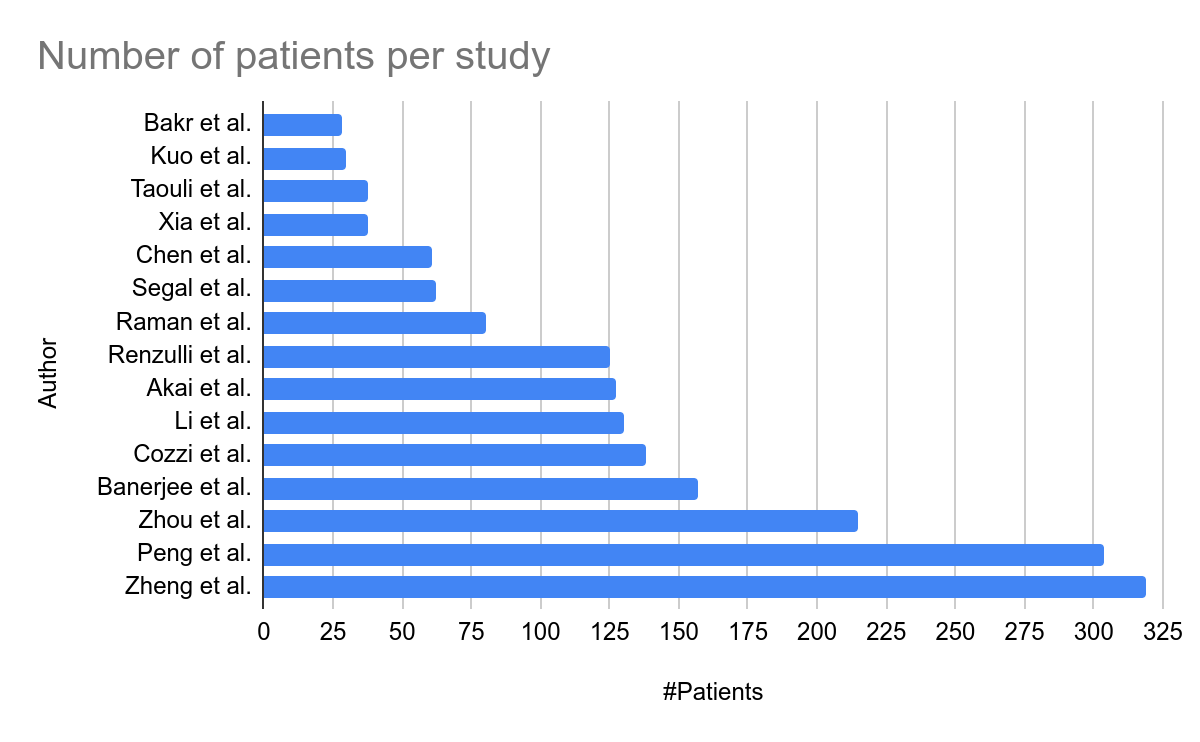
\includegraphics[width=4.41572in,height=2.72865in]{./images/image2.png}

The relatively low number of patients can be explained by the strong
inclusion criteria set within the studies (size and number of lesions,
baseline imaging examination within a given period of time before
initial treatment, \ldots{})

They were all built with data acquired on patients who underwent CT
examination, except one, that decided to mix data obtained from both CT
and MR examinations {[}\textbf{Taouli et al. \#45}{]}.

Regarding the CT scan protocol, only one study decided to use images
acquired before the injection of contrast medium {[}\textbf{ref Cozzi
\#1}{]}, whereas two other studies used images acquired at only one
phase (early arterial phase for \textbf{Raman et al. \#26}, and portal
venous phase for \textbf{Li et al. \#24}), and the remaining studies
analyzed multiphase images. Among them, four studies utilized images
acquired at both early arterial and portal venous phases {[}\textbf{ref
Zhou \#2, Chen \#23, Kuo \#29 and Zheng \#40}{]}, while the rest were
based on traditional triphasic images {[}\textbf{ref Akai, Banerjee,
Renzulli, Segal, Peng, Bakr, Taouli and Xia}{]}. Concerning the
acquisition protocols, early arterial phase images are most of the time
acquired around 30s after the injection of contrast agent (between 22
and 35s), and some studies used bolus tracking method to estimate the
best acquisition moment instead of using the same timing for all the
patients. Portal venous phase images are acquired between 45 and 70s
after the injection, and the delayed images obtained during an even
larger interval (between 90 and 300s after the injection).\\
Knowing that images are the key elements in the computation process of
the radiomics features, this high variation within the acquisition
protocols is the first reason why the standard \emph{HCR} pipeline
should be standardized.

Once the images acquired, the following step consists in selecting the
region of interest to compute the features, or evaluate the
physiological properties of the lesions to the naked eye.

\paragraph{ROI selection}\label{roi-selection}

The selection of the region/volume of interest and/or the assessment of
the physiological characteristics of the tumor is often performed by one
or multiple experienced radiologists.\\
This step of the pipeline was performed by only a single expert in rare
cases in the reviewed studies {[}\textbf{Xia, Akai}{]}, whereas it was
usually performed by two experts {[}\textbf{Zhou, Chen, Li, Raman, Kuo,
Renzulli, Segal, Zheng, Peng, Taouli}{]}.\\
When more than 1 expert is involved, the authors decided to implement
ways for quantifying the inter and intra-observer variability, such as
the \emph{ICC} (Intraclass Correlations Coefficient) {[}\textbf{Zheng,
Li}{]}, or the Cohen k statistics {[}\textbf{Banerjee, Renzulli}{]}.

Regarding now the selection of the ROI, we can separate the reviewed
studies by the type of features being extracted.

On one hand, when using imaging traits, it is common to use the whole
tumor to perform the evaluation. For example when evaluating the
vascular invasion, some features like the peritumoral enhancement need
to be estimated globally {[}\textbf{Renzulli et al., Banerjee et al.,
Segal et al., Kuo et al.}{]}.\\
On the other hand, when using computational features, the analysis can
be performed on the whole tumor or on a single slice. Some studies
decided to compute the features on the entire 3D ROI, as an example
\textbf{Cozzi} \textbf{et al.} used the entire tumor independently on
the tissues present within it, \textbf{Xia et al.} decided to separate
areas based on their textural properties as depicted below, but the
analysis remains global. Other studies placed everal ROIs all throughout
the tumor (3 ROIs for \textbf{Bakr et al.} and from 5 to 10 for
\textbf{Raman et al.}). However, the majority of the studies decided to
place the ROI at the largest cross-sectional area {[}\textbf{Li, Chen,
Zhou, Akai, Zheng}{]}.

\begin{figure}[ht!]
\centering
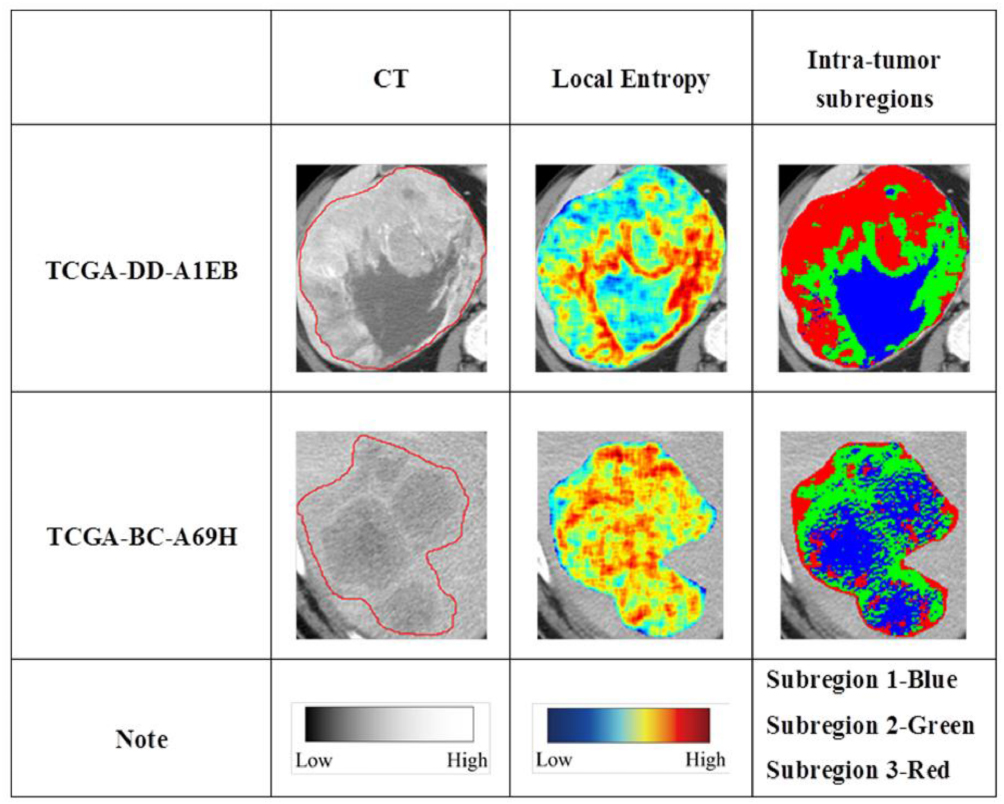
\includegraphics[width=4.34043in,height=3.46021in]{./images/image16.png}
\caption{Illustration of intratumor partition for two representative
patients (TCGA-DD-A1EB and TCGA-BC-A69H). The first column shows the
tumor outlines on the original CT image. The second column shows the
heatmaps of calculated local entropy on tumor images. The third column
shows the three subregions marked with different colors after intratumor
partitioning. \textbf{©Xia et al.} }
\end{figure}

Note that some studies decided to compute the features using both the
entire volume and the slice-wise approach (e.g. \textbf{Taouli et al.}
evaluated imaging traits globally and computed the ratio using a
slice-wise fashion, \textbf{Peng et al.} did the same in their study by
computing features using an ROI placed at the largest-cross sectional
area, and evaluating imaging traits globally).

Worth mentioning that before the computation of features, it is common
to filter the images using different kernel sizes, in order to enhance
different elements of the volumes such as the blood vessels for example.
All reviewed studies that computed quantitative features filtered their
images with a Laplacian of Gaussian algorithm with various sizes, as
depicted below {[}\textbf{Akai et al.}{]}.

\begin{figure}[ht!]
\centering
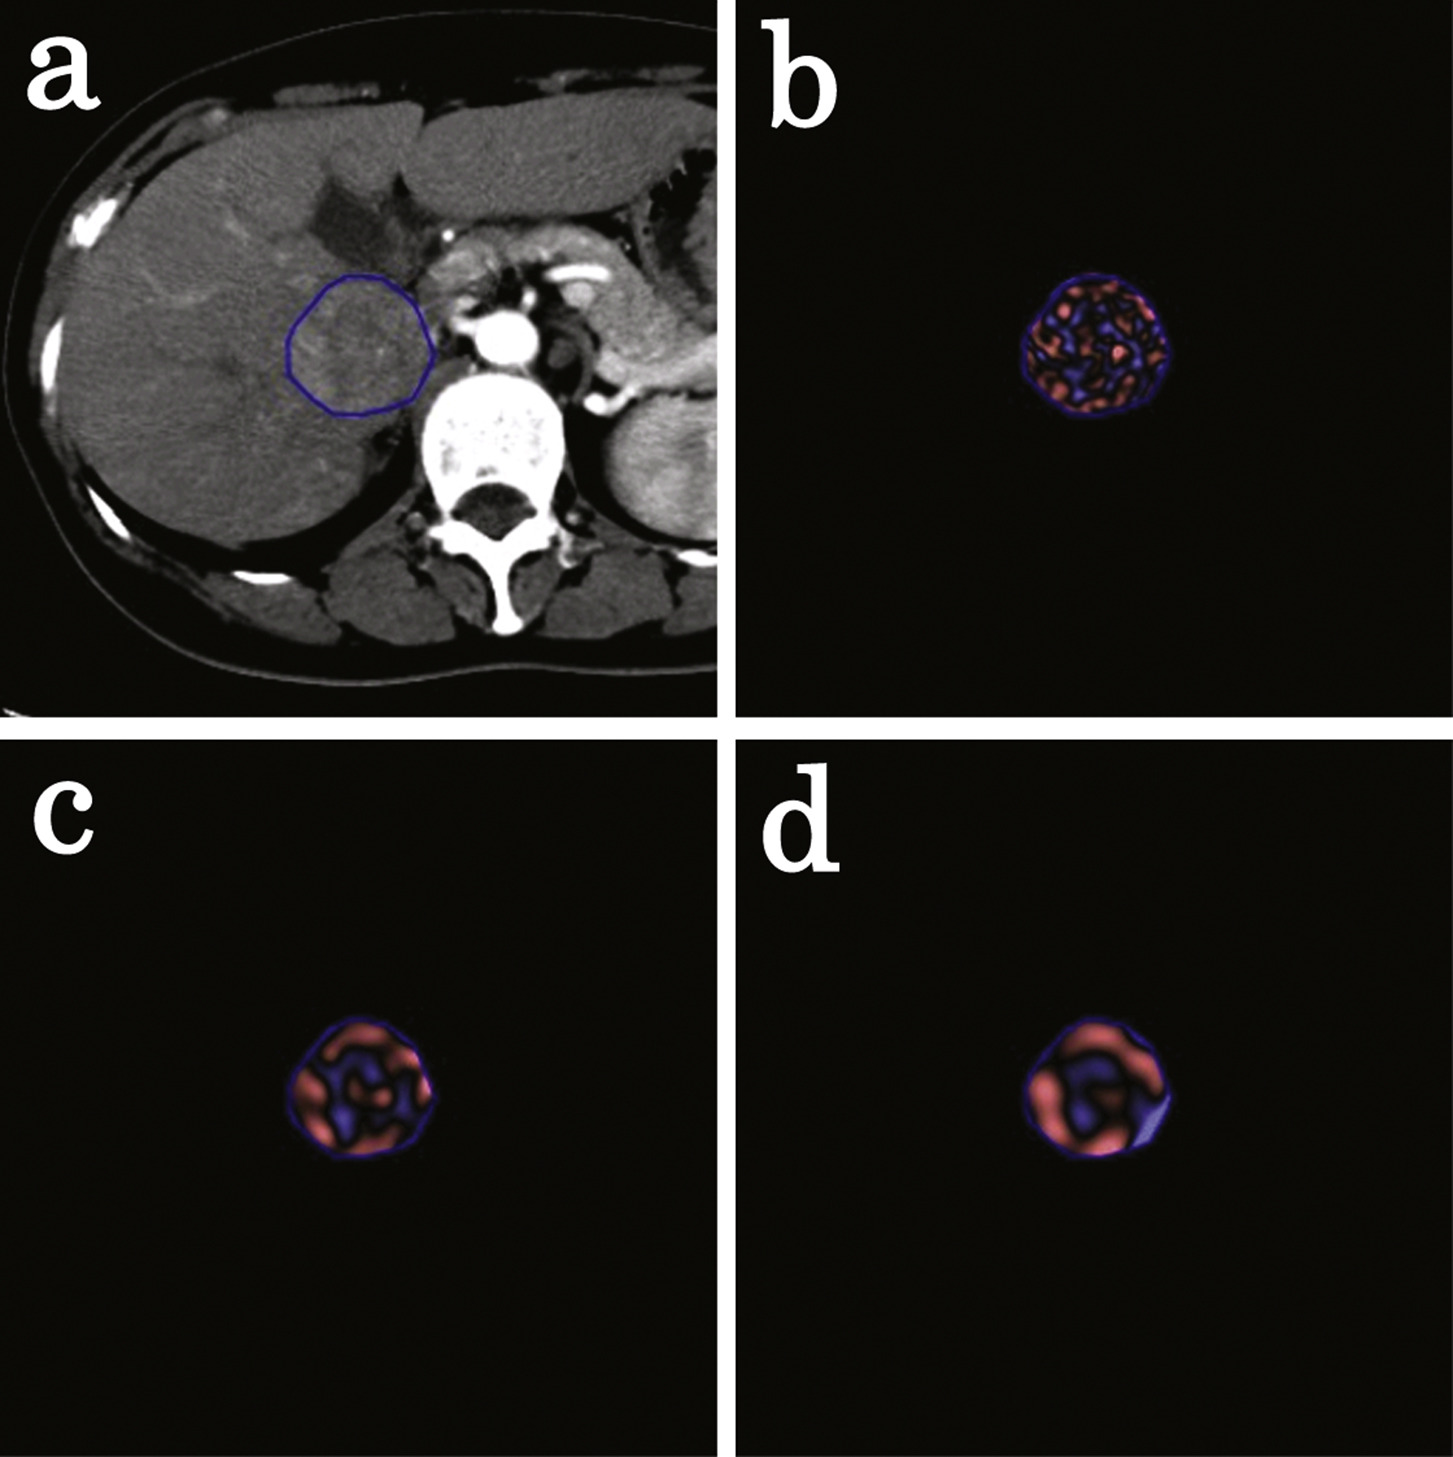
\includegraphics[width=3.50110in,height=3.51334in]{./images/image15.png}
\caption{ Screenshot of the CT texture analysis software. A polygonal ROI was
drawn on the tumor (a). Processed images using Laplacian of Gaussian
filters with SSF of 2 mm (b), 4 mm (c), and 6 mm (d) were automatically
generated. The images were displayed using a red or blue scale showing
negative or positive pixels, respectively. \textbf{©Akai et al.}}
\end{figure}

\paragraph{Features selection}\label{features-selection-1}

Once the ROI delineated and pre-processed, the following step consists
in extracting the features, and as explained previously, the choice on
which features to extract depends on the type of features the study is
going to rely on, quantitative or semantic.

In the case of quantitative features, the reviewed studies often decided
to focus on a single category of features (first-order, textural
features, higher-order\ldots{}), thus obtaining a relative small number
of features (27 for \textbf{Li et al.}, 32 for \textbf{Raman et al.}).
However, despite choosing a specific category of features, this number
can increase, when combining the native features with the spatial
filter, and the different contrast enhanced phases, as in \textbf{Akai
et al.} where a total 96 features are extracted from the initial 6
histogram-based features.

Some other studies decided to extract the maximum possible features by
combining the previously mentioned group of features, and thus obtained
300+ features, {[}\textbf{Zhou et al.}, \textbf{Peng et al., Bakr et
al.}{]}. The problem in this case, often called ``\emph{curse of
dimensionality}'', corresponds to a high number of features relative to
the number of individuals, and that can cause some troubles when further
training the predictable model.

When imaging traits are preferred to classical radiomics features, the
number of extracted characteristics is generally below 10, with a high
predominance of changes brought by the hepatocarcinogenesis, such as the
presence of internal arteries, or the wash-in wash-out effect (example
of imaging traits can be observed in the following figure). Even though
the number of extracted features is often small, they often correspond
to absence or presence of physiological properties that are sometimes
difficult to quantify and that will highly depend on the observer's
experience.

\begin{figure}[ht!]
\centering
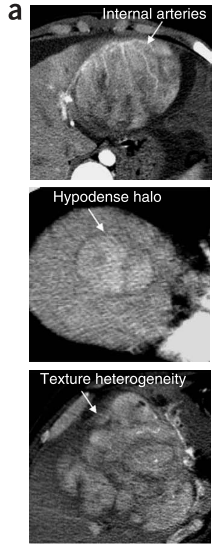
\includegraphics[width=1.13125in,height=2.82813in]{./images/image3.png}
\caption{{[}\textbf{Segal et al.}{]}
From top to bottom:
Internal arteries
Hypodense halo
Textural heterogeneity}

\end{figure}

\begin{figure}[ht!]
\centering
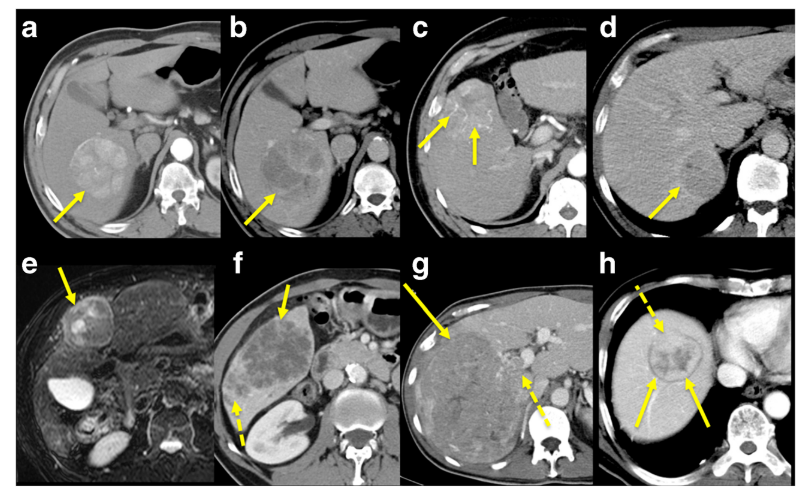
\includegraphics[width=4.67498in,height=2.86979in]{./images/image8.png}
\caption{{[}\textbf{Taouli et al. - Figure 1}{]}
(a,b) wash-in/wash-out pattern and mosaic appearance, without capsule/
pseudocapsule.
(c) internal arteries (arrows)
(d) pseudo-capsule (arrow)
(e) {[}MR image{]} hyperintense encapsulated with mosaic appearance
(arrow)
(f) internal necrosis and satellite lesions posteriorly (dashed arrow)
(g) right portal vein invasion (dashed arrow)
(h) extra-nodular growth anteriorly (dashed arrow)
}
\end{figure}


After the different features are obtained, the next step in the pipeline
consists in the selection of the features and the building of the
predictive model.

The vast majority of the reviewed studies decided to implement a
logistical regression model in order to assess the correlation between
features and the study endpoint. Among the existing methods,
time-related approaches such as the Cox regression model {[}\textbf{Li,
Banerjee, Zheng, Cozzi, Xia}{]} and the Kaplan-Meier survival analysis
{[}\textbf{Segal, Chen, Akai, Xia}{]} are the most commonly used,
especially because those are historical ways to predict the survival of
the patients.

Different statistical approaches were used by the studies that tried to
determine the link between selected features and study endpoints such as
the \emph{LASSO} (Least Absolute Shrinkage and Selection Operator)
algorithm {[}\textbf{Zhou, Peng, Bakr}{]}. In the other studies, other
approaches were implemented, for example, \textbf{Raman et al.}
performed a \emph{PCA} (Principal Components Analysis) followed by a
\emph{MANOVA} (Multivariate Analysis Of VAriances) to create clusters
among patients for the classification of hypervascular lesions, whereas
\textbf{Renzulli et al.} evaluated the positive and negative predictive
values of the selected features against the microvascular invasion
status of the patients.

The list of discriminant features per study is given in the tables
below, with a separation between quantitative and semantic features.


\textcolor{red}{\textbf{ADD TABLES HERE}}



\begin{table}{}
\textbf{Quantitative Features}\\ 
\emph{First Order Statistics}
\begin{itemize}
\item Shape {[}Cozzi{]}
\item Skewness {[}Akai, Li, Zhou{]}
\item Kurtosis {[}Akai{]}
\item Mean {[}Zhou, Raman, Cozzi{]}
\item Energy {[}Zhou, Cozzi{]}
\item Entropy {[}Peng, Akai{]}
\item Peak {[}Bakr{]}
\item Standard deviation {[}Xia{]}
\item Enhancement ratio {[}Taouli{]}
\item Tumor-Liver difference {[}Taouli{]}
\end{itemize} 
\emph{Second Order Statistics} 
\begin{itemize}
\item Gray Level matrices {[}Peng, Zheng, Cozzi{]}
\item Cluster prominence {[}Xia{]}
\end{itemize}
\emph{Higher Order Statistics}
\begin{itemize}
\item Wavelets {[}Chen, Li, Bakr{]}
\item Gabor {[}Chen, Bakr{]}
\end{itemize}
\emph{Morphological features}
\begin{itemize}
\item Tumor margin volume {[}Xia{]}
\item Tumor size\tnote{1}
\end{itemize}

\begin{tablenotes}
\item[1] {Tumor size in the two studies is not given as the exact volume, but
rather a classification of tumors in different categories (for example
the categories were smaller than 2cm, between 2 and 5 cm, and larger
than 5 cm in \textbf{Renzulli et al.})} {[}Renzulli, Taouli{]}
\end{tablenotes}
\end{table}

\begin{table}{}
\textbf{Semantic Features} \\ 
\emph{Two Traits Predictor of Venous Invasion}
\begin{itemize}
\item
  Internal arteries {[}Renzulli, Kuo, Peng, Segal, Banerjee, Taouli{]}
\item
  Hypoattenuating halos {[}Renzulli, Peng, Segal, Banerjee{]}
\end{itemize}
\emph{Intensity-related features}
\begin{itemize}
\item
  Peritumoral enhancement {[}Renzulli{]}
\item
  Presence of a Tumor-Liver difference {[}Banerjee{]}
\end{itemize}
\emph{Textural-related features}

\begin{itemize}
\item
  Non-smooth Tumor Margins {[}Renzulli, Kuo, Peng{]}
\item
  Infiltrative patterns {[}Taouli{]}
\item
  Mosaic appearance {[}Taouli{]}
\end{itemize}
\end{table}

Concerning the studies based on quantitative features we can notice that
first-order statistical features is the most common discriminant type,
which is normal because this group of histogram-based characteristics is
often implemented in the existing radiomics tools, whereas higher order
statistical features require more advanced knowledge to be implemented,
and often lack of interpretability.

Even though \textbf{Li et al.} decided to extract only Wavelet features
because they consider that the current way of computing textural
features is too dependent on the imaging acquisition settings, first and
second-order statistical features remain a good indicator of the
textural heterogeneity which is often correlated with the physiological
advances of the disease.

Worth also noting that imaging traits, often analyzed either alone, or
in combination with quantitative features, remain discriminant enough in
a lot of studies, because they are directly linked to the physiological
changes produced by the disease. Despite needing expertise to be
extracted, such as in \textbf{Segal et al}. where 32 different imaging
traits were analyzed, their predictable power drives us to consider them
in future radiomics studies and focus on a way to quantify them.

\paragraph{Study reproducibility}\label{study-reproducibility}

Although the majority of the reviewed studies obtained good predictable
results in regards with the wanted prediction task, their stability to
the experimental settings and their reproducibility remain questionable.

In 2017, \textbf{Lambin et al.} who remains one of the founders of the
radiomics fields {[}\textbf{ref Lambin 2012}{]} published a study
proposing a way to rethink the HCR pipeline and assess the robustness of
future radiomics studies {[}\textbf{ref Lambin 2017 RQS}{]}. This
assessment is performed thanks to the \emph{RQS} (Radiomics Quality
Score), which evaluates a total of 16 components with various weights.
The evaluation of the different components allows the computation of a
score ranging from 0 to 36 points where highest weights are given to
criteria allowing a better reproducibility of the study, such as the
prospective aspect of the study (7 points over 36) or the presence of a
validation step in the proposed workflow (5 points over 36, with a
penalty of 5 points when no validation at all is present).

Our reviewed studies were evaluated in regards with the \emph{RQS}, in
consensus with a medical research fellow (Wakabayashi Taïga)
{[}\textbf{ref Wakabayashi 2019}{]}.

The different scores per study can be found in the following table
(\href{https://docs.google.com/spreadsheets/u/0/d/10EHNALN2_6ZavU7049n6CwTfJO_vd6WBod64u8YNbHg/edit}{\emph{link}}).

The mean obtained \emph{RQS} by the reviewed studies was 8.73 +/- 5.57
points, which corresponds to less than 23\% of the maximal possible
score, and only one study obtained a more than 50\% of the maximum
points, which translates the lack of robustness of the current
\emph{HCR} state-of-the-art studies applied to the \emph{HCC}.

The table below allows us to see the most respected criteria in regards
with the RQS guidelines.

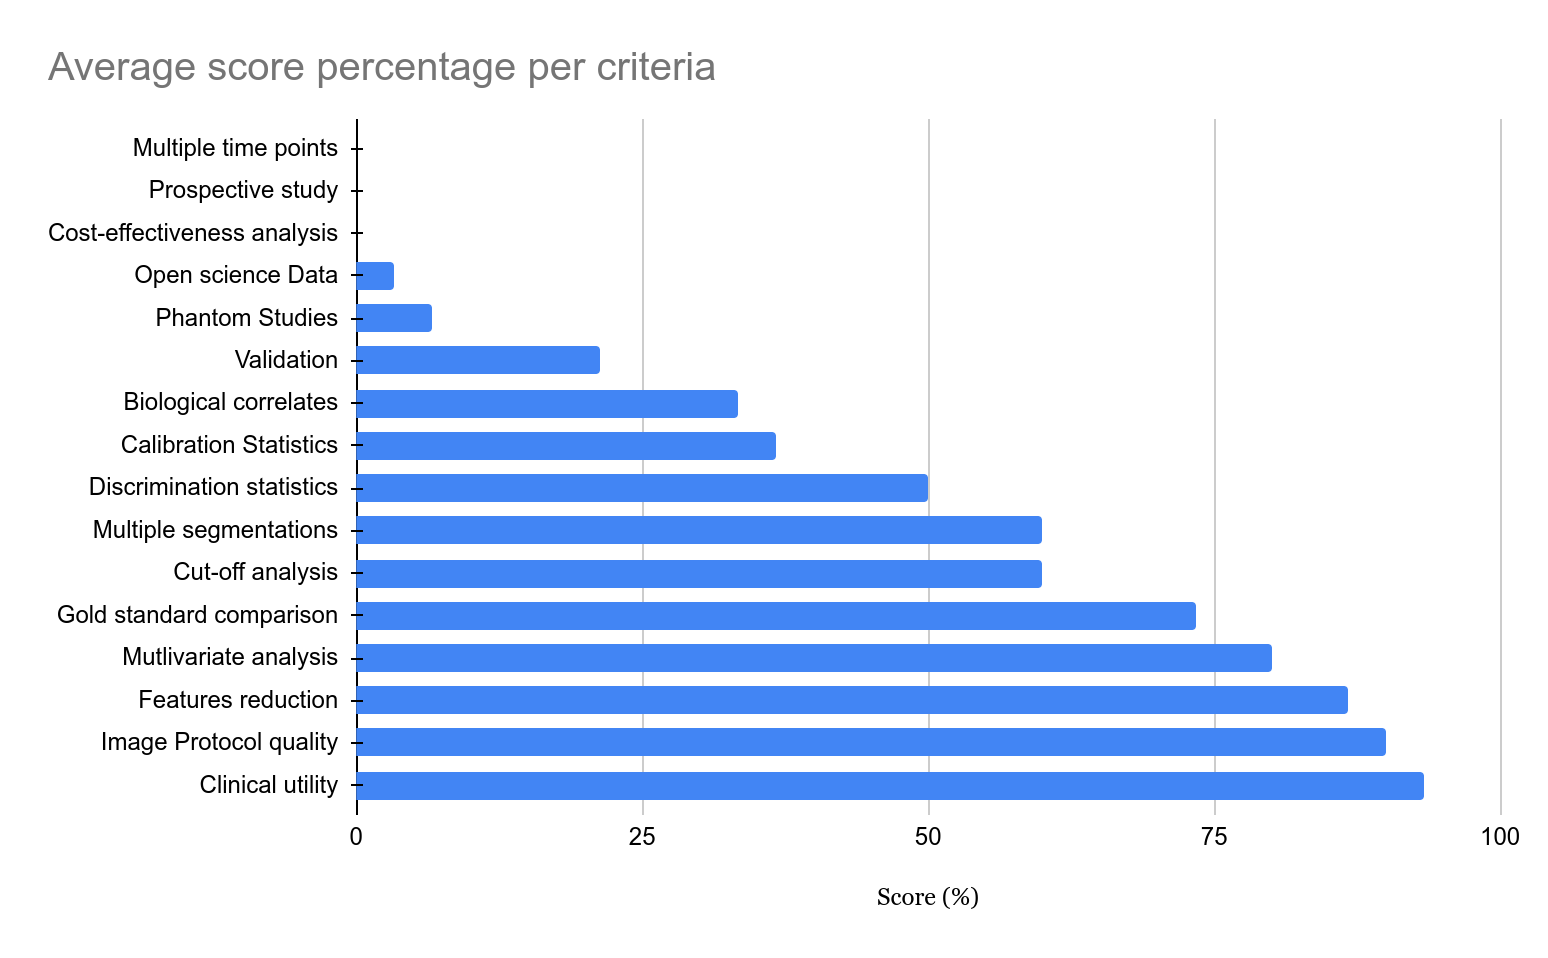
\includegraphics[width=6.26772in,height=3.87500in]{./images/image13.png}

The criteria the less respected by the different reviewed studies were
all those related with the reproducibility and the robustness. Among
them, the analysis of images acquired at multiple times, the
implementation of phantom studies to detect inter-scanner differences
and features sensitive to those settings, or even the prospective design
of the studies that will ensure inclusion of patients undergoing the
same protocols were almost always neglected.

Even though the different reviewed studies obtained successful results
in regards with the wanted task, their robustness relative to the
experimental settings and their reproducibility can be questioned,
especially when analyzing their results obtained on the radiomics
quality scoring system {[}\textbf{Lambin 2017}{]}.

One way to allow a better reproducibility for the future radiomics
studies is to fulfil the maximum possible criteria introduced by the
\emph{RQS} standard, and to use standard ways to compute the
quantitative features, thanks to open-source libraries such as
pyradiomics
{[}\href{https://pyradiomics.readthedocs.io/en/latest/}{\textbf{\emph{van
Griethuysen et al.}}} \textbf{2017}{]}. Another way is to reduce as much
as possible the impact of human-based interpretation in the \emph{HCR}
workflow. This can be done by replacing the hand-crafted annotations,
and the engineered process of features computation and selection by a
standardized, automated and data-driven pipeline, similar to what is
performed in more recent \emph{DLR} studies.

\subsection{Deep Learning Radiomics}\label{deep-learning-radiomics}

In this section we will first present the differences between the
\emph{HCR} and the \emph{DLR} strategies, before describing in detail
the \emph{DLR} concept. We will then present the different reviewed
studies tackling liver-related problems using a \emph{DLR} approach. We
will outline the different steps of their pipelines such as the use of
multiphasic images, the way they incorporated experts' annotations and
their choice regarding the deep network architectures.

\subsubsection{Difference between HCR and
DLR}\label{difference-between-hcr-and-dlr}

Being a young field, radiomics starts to mature when applied to several
organs such as the lungs or the breast, but it still struggles when
applied to the liver, especially because of the scarcity of available
data and the complexity of its anatomy.

As exposed previously, the first studies targeting liver cancer almost
always rely on hand crafted features (\emph{HCR} : Hand-Crafted
Radiomics).

The main limitation observed is the lack of reproducibility originating
from engineered features, that sometimes result from complex processes
which can be difficult to imitate, and often fail to work on different
databases.

\emph{HCR} rely on manual or semi-automatic expert annotations, which
often require a complex and time-consuming process, that also provide
several constraints, such as the poor inter-expert reproducibility.

The extracted features are not necessarily relevant to encode the
observed structure, it is needed to increase their number, hence
requiring a complex dimensionality reduction step.

Another limitation is the difficulty to find the perfect association
between features extraction, selection and the statistical analysis used
to reach the wanted target.

Those limitations, and the rise of new computational resources
associated with the emergence of deep learning techniques allowed the
development of a new branch in the radiomics field, called \emph{DLR}
(Deep-Learning Radiomics) {[}\textbf{ref Afshar et al. 2019}{]}.

\subsubsection{DLR workflow}\label{dlr-workflow}

In this branch of radiomics, the features are extracted through a
deep-learning process, avoiding a manual extraction.

A neural network can be trained to generate the most relevant features.
These features can either be kept in the network for the final
pathological target prediction, or used as input in a different model
(such as a SVM or a RF).

Compared to the \emph{HCR}, no prior knowledge is required, and the
features can be extracted in an end-to-end manner, using only the raw
images as input, and without necessarily providing any segmentation. It
has also been demonstrated that performances of those networks increase
with the size of the training dataset {[}\textbf{ref Cheng et al.
2016}{]}.

Eliminating the segmentation phase when evaluating the diagnosis, allows
to reduce the workload of experts, and provides a solution to the
observer-dependency.

When training \emph{DLR} networks, the original image can be combined
with the segmentation or any other pre-processed step result such as the
gradient image for example {[}\textbf{ref Sun et al. 2017}{]} to improve
the relevance of the extracted features.

Generally, \emph{DLR} studies can be classified depending on the type of
input used, the training strategy or the type or architecture choosed to
extract the features.

As input, deep radiomics networks can consider 2D slices independently,
however this technique does not bring sufficient information since the
decision mainly depends on the entire volume of interest.

The different outputs obtained in a slice-wise fashion can be fused to
get a volume-wise decision. The volume by itself can also directly be
used as input, however it can raise several issues such as the size of
the voxels or the slice thickness. Finally, the classification can be
performed by considering a series of volumes corresponding to the entire
examination of the patient {[}\textbf{ref Shen et al. 2016}{]}, but here
again the question regarding the normalization of the input can be
raised.

Once the type of input is chosen, the studies differ depending on the
training strategy. The networks can be trained \emph{from scratch} using
only the available data or a pre-existing architecture can be utilized.
In the first case, the obtained network will be specific to the wanted
task, but this specialization can also lead to troubles such as
overfitting or the sensitivity to imbalance data.

The impact of those problematics can be limited with the help of data
augmentation (use of existing data to generate new artificial samples)
{[}\textbf{ref Kumar et al. 2017}{]}, multi-task training (where the
number of parameters is limited by the training of several task using
the same network) {[}\textbf{ref Jamaludin et al. 2016}{]} or the
incorporation of the proportion of each class present in the data when
building the cost function {[}\textbf{ref Jamaludin et al. 2016}{]}.

The other strategy consists in using an architecture pre-trained most of
the time on natural images, and then re-train only a specific part on
the wanted task {[}\textbf{ref Echaniz, Huynh, Paul 2017- 2016}{]}. It
is worth noting that this type of training constrains the pipeline to be
slice-wise since existing architectures are often pre-trained on 2D
images.\\
Finally, the features can be extracted using either a supervised or an
unsupervised approach. In the supervised case, the most commonly used
networks are based on convolutional layers (\emph{CNN}), followed by one
or multiple dense layers to predict the output class. While the network
is trained to perform the classification, the features are extracted
either after a fully connected layer {[}\textbf{ref Paul et al.
2016}{]}, or after one of the convolutional layers {[}\textbf{ref Li et
al. 2017}{]}.\\
Other variants that are also built with convolutional layers as key
components can also be implemented (\emph{RNN}, \emph{LSTM} or
\emph{Capsule Net}). Their goal is to get rid of the limitations caused
by the input format that need to be fixed, and by the difficulty to
consider an entire 3D volume during the training {[}\textbf{ref Azizi et
al. 2018}{]}.

In the unsupervised case, the objective is to let the extracted features
be responsible for the data distribution, so that new cases can be
created following this distribution. The most commonly used architecture
in this case is the \emph{auto-encoder}, made up with a part that
contracts the information (encoder), in order that the most useful one
is conserved to regenerate the original data (decoder). Auto-encoder can
be built on top of convolutional layers {[}\textbf{ref Echaniz et al.
2017}{]}, or trained with the aim of being insensitive to the noise
added to the input data {[}\textbf{ref Sun et al. 2017, Kim et al.
2016}{]}. Following the same principles which are to reconstruct the
original input data using only the most relevant features, some studies
implemented \emph{DBN} (Deep Belief Networks) \textbf{{[}ref Sun et al.
2016{]}} or Deep Boltzmann Machines {[}\textbf{ref Suk et al. 2014}{]}.

Some studies are referred to as hybrid, when features are combined with
other sources of data (combination of different modalities
{[}\textbf{ref Oikonomou et al. 2018}{]} or association with clinical
data such as genomic data {[}\textbf{ref Emaminejad et al. 2016}{]}), or
when only a part of the pipeline implements deep learning methods,
either for the extraction of the features {[}\textbf{ref Paul et al.
2016}{]} or when the decision is taken with a fusion between \emph{HCR}
and \emph{DLR} features {[}\textbf{ref Huynh et al. 2016}{]}.

\subsubsection{DLR applied to the liver}\label{dlr-applied-to-the-liver}

Even though the number of studies targeting the liver is increasing, the
vast majority of them can be categorized as \emph{HCR}, and only a few
are currently based on deep learning.

The main reason behind that is the late emergence of deep learning and
the recent outbreak of new architectures and concepts that are often
first developed and evaluated in other fields than the medical imaging
one (e.g. Residual Network, DenseNet, Capsule Net).

\paragraph{Study Endpoint}\label{study-endpoint}

Within the reviewed \emph{DLR} studies, the majority of them are
targeting a diagnosis, either the classification of \emph{FLLs} (Focal
Liver Lesions) {[}\textbf{Yamada et al. 2019, Wang et al. 2018, Yasaka
et al. 2018, Liang et al. 2018}{]} or the estimation of the fibrosis
stage {[}\textbf{Yasaka et al. 2018}{]}, when two of them focused on the
response to treatments, either for recurrence after resection
{[}\textbf{Wang et al. 2019}{]} or the response after \emph{TACE}
{[}\textbf{Peng et al. 2019}{]}.

We selected the studies using \emph{CT} images to perform their
analysis, and realized that the vast majority of them used multiphasic
images to perform their research, knowing that the evolution of contrast
medium is often correlated with the pathological features of the liver
as mentioned in the \textbf{Medical Context}. The only one that used
single phase images, was the one targeting an estimation of the fibrosis
stage, and their method was based on portal phase images only
{[}\textbf{Yasaka et al. 2018}{]}. Regarding the multiphasic studies,
there is no consensus about the delay between the injection of the
contrast agent and the acquisition of the different phases. They tend to
prefer triphasic acquisition, with images acquired before the injection
of contrast agent, at early arterial phase and a third phase, either
portal venous {[}\textbf{Wang et al. 2018, Liang et al. 2018, Wang et
al. 2019}{]} or a delayed one {[}\textbf{Yamada et al. 2019, Yasaka et
al. 2018}{]}. \textbf{Peng et al.} decided to get rid of the \emph{NECT}
(non-contrast-enhanced) phase, but still chose a triphasic acquisition
(\emph{AR, PV, DELAY}).

\paragraph{Image processing pipeline}\label{image-processing-pipeline}

Concerning the image processing pipeline, the data used to train the
deep networks are most commonly selected via placement of a bounding box
by the experts around the hepatic lesion, before a registration between
the different phases in case of multiphasic acquisition to counter the
effects of body motion and/or breathing.

The manual placement of the \emph{ROIs} is usually done by one or more
experts on the raw image {[}\textbf{Yamada et al 2019, Wang et al. 2018,
Yasaka et al. 2018a, Wang et al. 2019, Yasaka et al. 2018b}{]}, and only
one study decided to perform an automatic segmentation of both the
parenchyma and the lesion with the application of a random-walker
algorithm, before being checked by experts {[}\textbf{Liang et al.
2018}{]}. When the method is based on a 2D approach, selected images are
often those presenting the maximal cross-sectional proportion of the
lesions, except one study targeting the estimation of the fibrosis
stage, that centered the \emph{ROI} so it displayed the ventral aspect
of the liver {[}\textbf{Yasaka et al. 2018b}{]}. Only one study
incorporated 3D information in their pipeline, but they also started the
placement of the \emph{VOI} with the slice presenting the maximal
proportion of tumor, and extended it to adjacent slices {[}\textbf{Yang
et al. 2019}{]}.

After placing a bounding box, the images are registered either manually
{[}\textbf{Yamada et al. 2019, Wang et al. 2018, Wang et al. 2019}{]} or
via the application a non rigid registration with anatomical constraints
{[}\textbf{Liang et al. 2018}{]}. No real registration was mentioned for
two studies {[}\textbf{Peng et al. 2019, Yasaka et al. 2018b}{]} but
Yamada et al. evaluated the effects of the registration in the
prediction performances of their networks (as depicted in the figure
below), and after training several networks with misregistered data
(shifted, rotated, skewed) they concluded that in the vast majority of
the cases, no statistical significance can be found between the
performances of the networks trained with manually registered data and
those of the networks trained with misregistered data {[}\textbf{Yamada
et al. 2019}{]}.

\begin{longtable}[c]{@{}l@{}}
\toprule
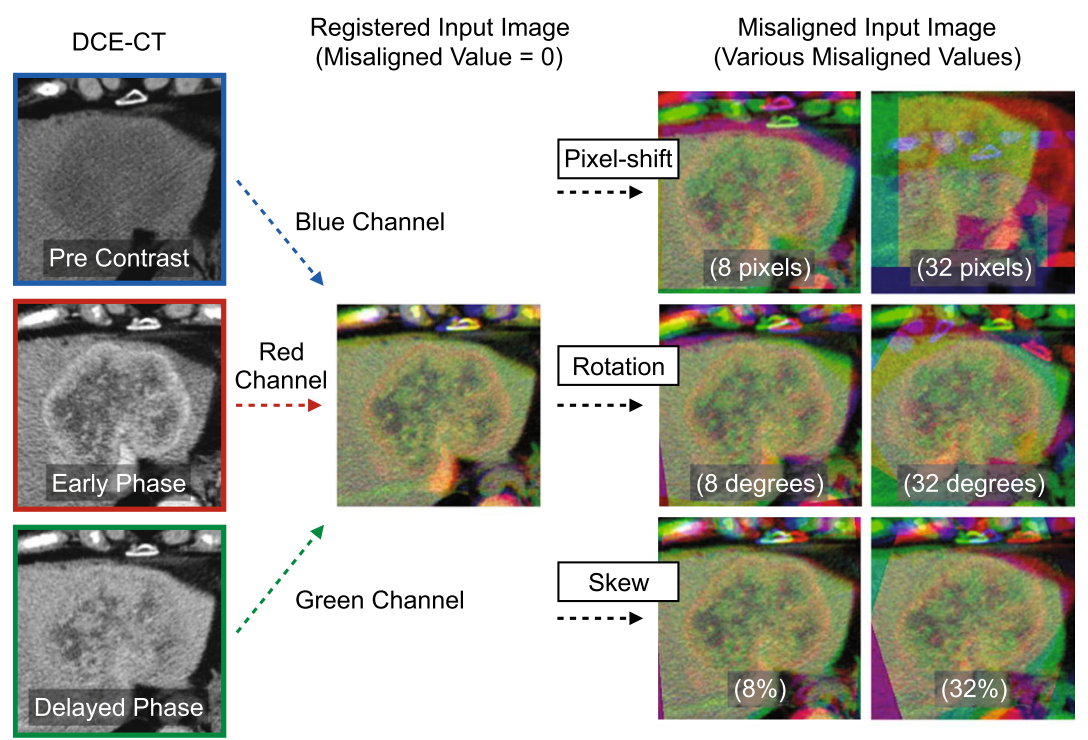
\includegraphics[width=6.11458in,height=4.15278in]{./images/image12.png}\tabularnewline
\midrule
\endhead
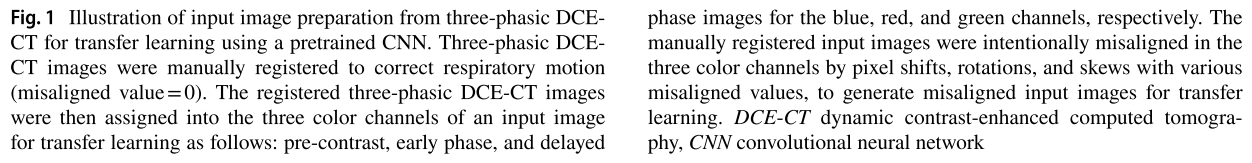
\includegraphics[width=6.11458in,height=0.79167in]{./images/image1.png}\tabularnewline
\bottomrule
\end{longtable}

Worth noting that some studies performed their analysis on cropped or
resized JPEG images {[}\textbf{Yasaka et al. 2018a, Yasaka et al. 2018b,
Wang et al. 2019}{]}. This choice might cause loss of data, since RGB
channels are encoded with 256 values whereas the raw data is used
elsewhere, where the liver HU intensities are often in the range
{[}-100, 400HU{]}.

\paragraph{Training strategies}\label{training-strategies}

Finally, in the reviewed studies, only two of them combined images with
clinical data {[}\textbf{Yasaka et al. 2018b}, \textbf{Wang et al.
2019}{]}, whereas the other only used image data, which is
understandable because clinical data are often difficult to retrieve,
and can also be difficult to integrate in a deep network, as illustrated
in the figure below.

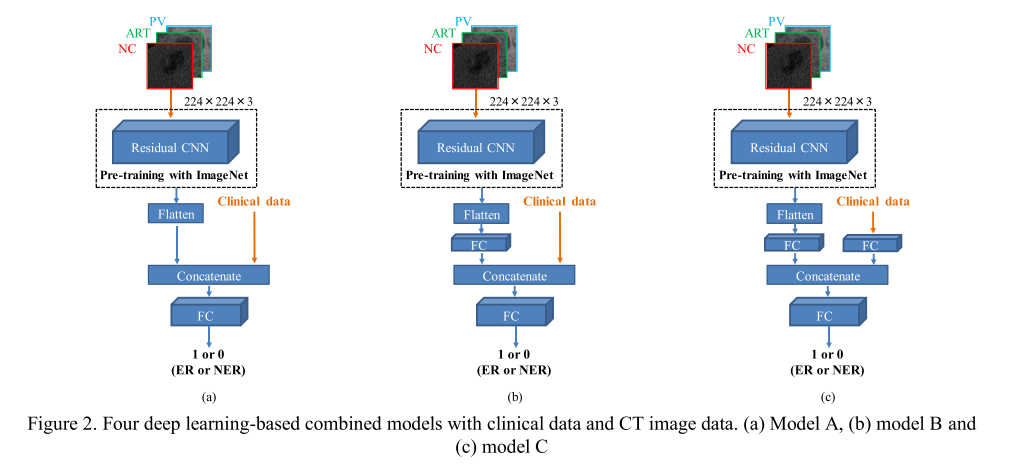
\includegraphics[width=5.60113in,height=2.56796in]{./images/image5.png}

The reviewed studies differ mainly in the way they built their deep
architecture.

In most of the cases, convolutional layers are used for the extraction
of the most discriminant features. The main question being whether to
use a pre-trained network or to train a network from scratch. In the
case of fine-tuning, the most commonly used architectures are
\emph{AlexNet} and \emph{ResNet} {[}\textbf{Wang et al. 2018, Yamada et
al. 2019, Wang et al. 2019, Peng et al 2019}{]}, but it is also usual to
compare the results obtain by different pre-trained architectures
{[}\textbf{Wang et al. 2019a, Yamada et al. 2019}{]}. The general method
is to recycle an architecture trained on a huge dataset such as
ImageNet, freeze the weights of the early layers (responsible for the
high levels features), adjust and train the last layers on the current
database to be more specific.

An illustration of this process can be found in the figure above
{[}\textbf{Yamada et al. 2019}{]}.

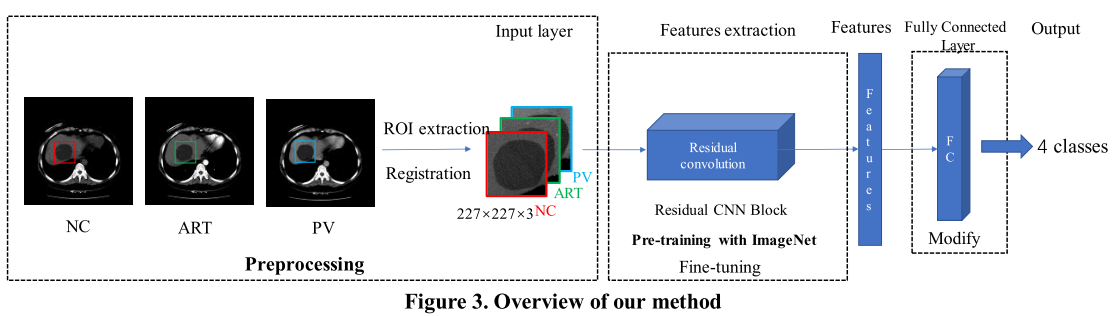
\includegraphics[width=6.26772in,height=1.77778in]{./images/image6.png}

The rest of the reviewed studies created a custom architecture and
trained it from scratch {[}\textbf{Yasaka et al. 2018a, Yasaka et al.
2018b, Liang et al. 2018}{]}.

Two of them used classical convolutional layers followed by max pooling
layers, early in the network to extract relevant features, as depicted
in the figure below {[}\textbf{Yasaka et al. 2018a, Yasaka et al.
2018b}{]}.

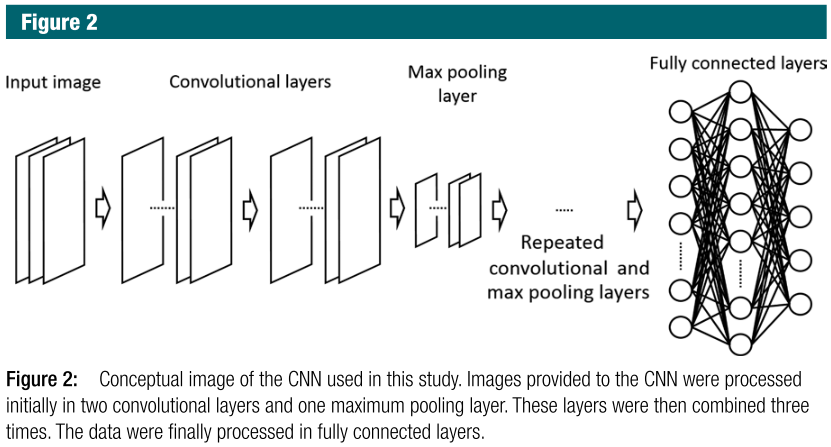
\includegraphics[width=4.77665in,height=2.57082in]{./images/image10.png}

Since multiphasic studies often stacked the different phases as channels
to feed the deep network, one study decided to extract the temporal
information through a different paradigm by using \emph{LSTM} (Long
Short Term Memory) layers {[}\textbf{Liang et al. 2018}{]}. As depicted
below, their architecture first extracted the features using what they
called a ``ResGLBlock'' per phase, with two scaled data as input (a
large one with the entire lesion, and a smaller one with finer details),
and conserved the temporal information via bidirectional \emph{LSTM}
layers.

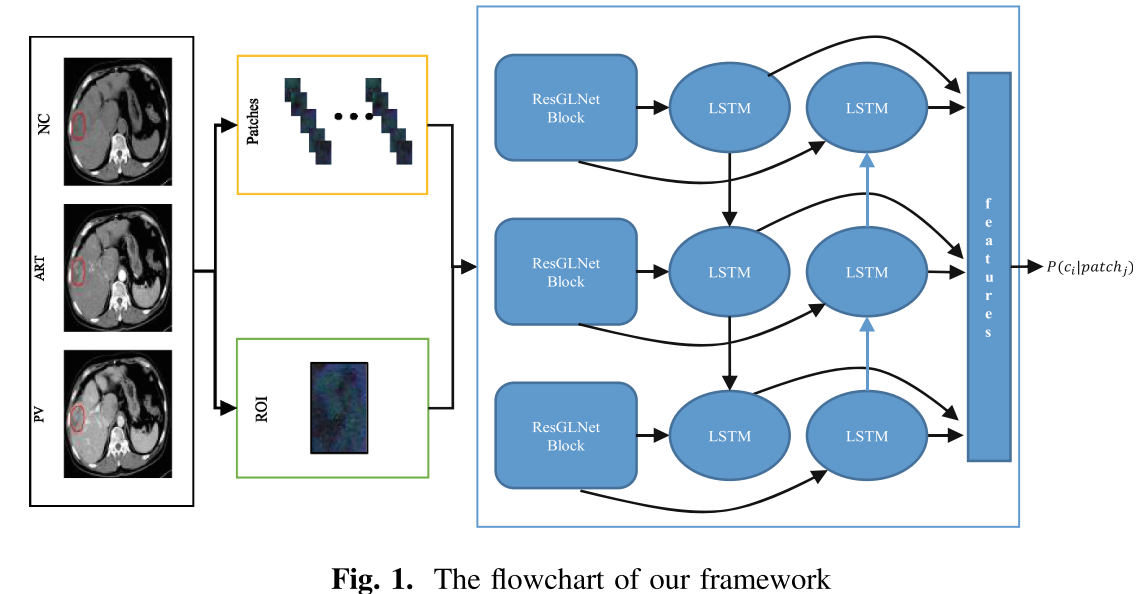
\includegraphics[width=5.07513in,height=2.63463in]{./images/image7.png}

When using a pre-trained architecture, the input size is often dictated
by the native architecture (224x224x3 for example for the ResNet
architecture {[}\textbf{Peng et al. 2019, Wang et al. 2019b}{]}), and
the different studies need to resample their inputs to fulfill those
requirements, which can sometimes affect the performances of the
network, whereas custom architectures allow a usage of custom sizes
{[}\textbf{Yasaka et al. 2018a, Yasaka et al. 2018b, Liang et al.
2018}{]}. However, the size of the lesions or other extracted \emph{ROI}
is often different from one patient to the other, therefore, this
problem is still open.

One way to render the deep networks robust to those changes is through
data augmentation. Yasaka et al. 2018a for example trained the network
with patches cropped at different resolutions from the initial lesion
\emph{ROI} after application of standard geometrical transformations
such as rotation or shift {[}\textbf{Yasaka et al. 2018a}{]}. The same
process of extracting different patches from an initial ROI is performed
by two other studies, where the goal is also to balance the different
classes {[}\textbf{Yasaka et al. 2018b, Peng et al. 2019}{]}.

The networks are then usually trained in a cross validation fashion
{[}\textbf{Yamada et al. 2019, Yasaka et al. 2018a, Yasaka et al. 2018b,
Wang et al. 2019}{]}, or validated on external dataset {[}\textbf{Peng
et al. 2019}{]} to be less affected by the effect of randomness, and to
be less prone to overfitting.

\paragraph{Performances}\label{performances}

Regarding their performances on their testing sets, the different
studies concluded first that fine tuning allows an improvement in the
accuracy of the \emph{DLR} network, when compared to training from
scratch (e.g. Wang et al. reported an improvement from 83.7 to 91.2\%
regarding the classification accuracy of their model when using a
pre-trained network) {[}\textbf{Yamada et al. 2019, Wang et al.
2018}{]}. Several studies also demonstrated that multiphase images
increase the performances or the \emph{DR} networks, when compared to
single phase input only {[}\textbf{Yasaka et al. 2018a}{]}. Instead of
training the \emph{DR} networks only with images, it is possible to
combine them with clinical data which can be difficult to collect, and
challenging to integrate in a deep architecture, but are proven to
improve the accuracy of the networks in some cases {[}\textbf{Wang et
al. 2019}{]}.

Reported results showed moderate to good accuracy for the wanted tasks.
For example, the reported mean accuracy is above 0.90 for the studies
targeting a classification between Focal Nodular Hyperplasias, Cysts,
HCC and Hemangioma (0.91 in both \textbf{Liang et al. 2018 and Wang et
al. 2018}), and it slightly drops to 0.84 when more complex categories
are integrated (iCC, combined HCC and difference between HCC and early
HCCs) {[}\textbf{Yasaka et al. 2018a}{]}. Another study performed the
classification between HCCs and non HCCs, by additionally incorporating
the differentiation stages for the HCC group, but still had comparable
performances than experienced radiologists in the diagnostic
performances {[}\textbf{Yamada et al. 2019}{]}.\\
The study targeting the estimation of the fibrosis stage reported
results less accurate than those obtained using elastography data
(\emph{MRE}: Magnetic resonance elastography or \emph{TE}: Transient
elastography), but they were the first to perform this analysis on CT
images, and their results could be improved with the inclusion of
volumetric information, and other sources of data. {[}\textbf{Yasaka et
al. 2018b}{]}.

Finally, the studies predicting a response to a treatment reported a
high accuracy with an AUC of 0.82 when predicting the recurrence after
TACE {[}\textbf{Wang et al. 2019}{]}, and accuracy above 0.83 in the two
external validation sets when estimating the response of TACE in HCC
{[}\textbf{Peng et al. 2019}{]}.

Those results still can be improved, especially by increasing the size
of the cohort, or by replacing the manual placement of the bounding
boxes with an automatic segmentation method in order to reduce the
dependency to single or multiple experts {[}\textbf{Yasaka et al. 2018b,
Peng et al. 2019}{]}.

As a conclusion, the different reviewed studies tend to agree on the
fact that a multiphase analysis is necessary to precisely describe and
encode the pathological features of the disease. For the rest of the
pipeline, no real consensus exists but several strategies are
implemented especially to compensate for the small size of the
databases. Worth also noting that the reviewed studies correspond to the
first DLR liver-related applications, therefore, they tend to tackle the
less complex problems such as the FLLs classification. With future
improvements regarding DL applied to the medical imaging field, and with
more publicly available data, the next DLR liver-related studies will be
ready to tackle more complex challenges.

\newpage
	\bibliographystyle{unsrt}
	\bibliography{../biblio}

\end{document}
